% register + bus diagram
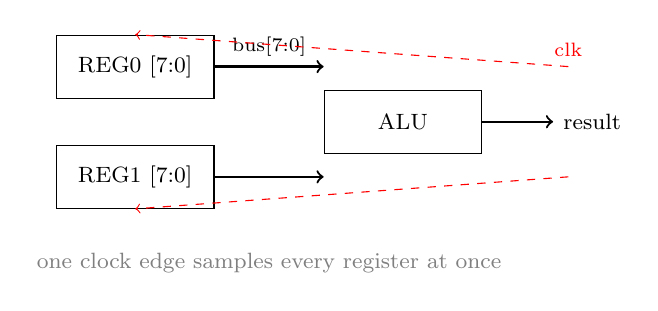
\begin{tikzpicture}[font=\footnotesize, reg/.style={draw, minimum width=2.0cm, minimum height=0.8cm}]
\node[reg] (r0) at (0,0) {REG0 [7:0]};
\node[reg] (r1) at (0,-1.4) {REG1 [7:0]};
\node[reg] (alu) at (3.4,-0.7) {ALU};
\draw[->, thick] (r0.east) -- node[above, font=\scriptsize] {bus[7:0]} (alu.west |- r0.east);
\draw[->, thick] (r1.east) -- (alu.west |- r1.east);
\draw[->, thick] (alu.east) -- ++(0.9,0) node[right] {result};
\draw[->, dashed, red] (5.5,0) node[above, font=\scriptsize] {clk} -- (r0.north);
\draw[->, dashed, red] (5.5,-1.4) -- (r1.south);
\node[gray] at (1.7,-2.5) {one clock edge samples every register at once};
\end{tikzpicture}
